\paragraph{Milling}

\begin{figure}[ht]
    \centering
    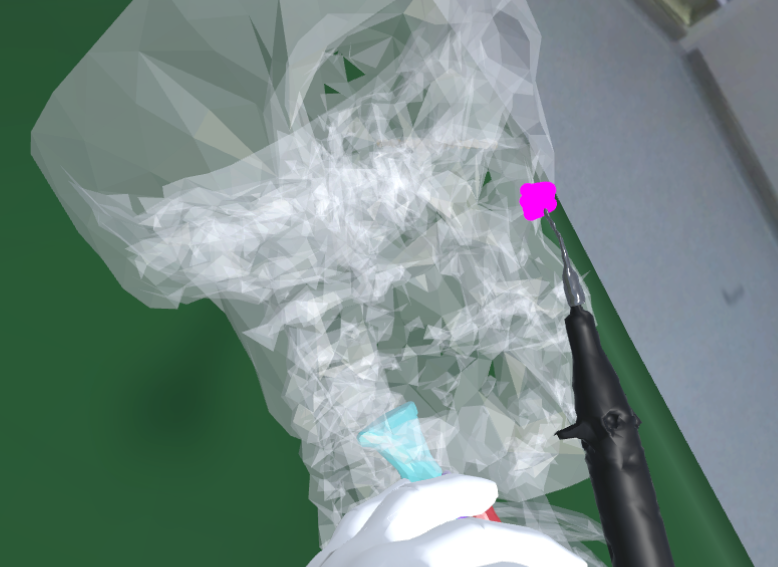
\includegraphics[width=200px]{images/implementation/features/procedures/piezo.png}
    \caption{\label{fig::FeaturePiezo}Milling procedure. Holding down the trigger button will draw little spheres until the button is released. The resulting object represents the volumetric space which is to be milled.}
\end{figure}

The \textbf{milling} operation is performed with the by grabbing the piezo instrument.
The indicator for the piezo is at the tip of the instrument, indicating which area will be milled.
While the "perform" button is being held down, little spheres are being drawn at the tip of the instrument \ref{fig::FeaturePiezo}.
When the button is released, the shapes are combined into a single 3D model and added as a project step.
The resulting object represents the volumetric space which has to be milled in the procedure.
The procedure can be reconstructed by "milling" the same 3D space in the virtual operating room.